\subsubsection{\atlasC{Prospects for resonant double Higgs production in the 4 b-quarks final state at the HL-LHC}}
\contributors{S. Willocq and A. Miller, ATLAS}
%{\bf Author(s): S. Willocq and A. Miller, ATLAS}

The projection study in \citeref{ATL-PHYS-PUB-2018-028} and summarized here uses the search for high-mass spin-2 KK gravitons decaying into two Higgs bosons, $HH$, as a benchmark, with each of the Higgs bosons decaying to $b\bar{b}$, thereby yielding 
a final state with two highly boosted $b\bar{b}$ systems, which are reconstructed as two large-radius jets.
The following strategy is followed to obtain sensitivity estimates at the HL-LHC: 
(i) signal and background mass distributions for the pair of candidate Higgs bosons in the event 
are taken from the most recent ATLAS data analysis at $\sqrt{s}$ = 13~TeV \cite{ATLAS-Resonance-4b} and scaled to 3000~fb$^{-1}$;
(ii) simulated signal and background mass distributions are used to 
derive mass-dependent scaling functions to extrapolate the distributions
from $\sqrt{s}$ = 13~TeV to 14~TeV;
(iii) simulated signal and background mass distributions are used for further scaling
of the distributions to reproduce the impact of additional selection criteria
not included in Run 2 searches. 

The dominant background for the 13~TeV data analysis stems from multijet production. 
This background source is estimated directly from data in that analysis and represents about 
80\%, 90\%, and 95\% of the total background in the signal region for events with
2, 3, and 4 $b$-tags (the classification of events based on the number of $b$-tags is described below).
The remaining source of background originates almost completely from $\ttbar$ production.
The shape of the dijet mass distribution for $\ttbar$ events is taken from MC samples. 
The normalization of the $\ttbar$ background in \citeref{Aaboud:2018knk} 
is extracted from a fit to the leading large-$R$ jet mass distribution in the 13~TeV data.
Samples of simulated multijet background events are generated to derive scaling functions
to be applied to the background predictions from the 13~TeV data analysis.
These samples are generated at both $\sqrt{s} = 13$~TeV and $\sqrt{s} = 14$~TeV.
Two different sets of MC samples are used to study the impact of differences in jet
flavor composition on the multijet background scaling functions.
The first set of events corresponds to the $2 \to 2$ processes $pp \to jj$ (with $j = g$ or $q$)
generated with \PYTHIA~8 with truth jet $\pt$ in the range between 400 and 2500~GeV.
The second set of events corresponds to the $2 \to 4$ processes $pp \to bbbb$ generated
with \MGvATNLO  requiring $b$-quarks to have $\pt$ above 100~GeV and the events are required to have at least one $b$-quark 
with $\pt$ above 200~GeV.

%The truth-level events generated to derive scaling functions are processed with 
%a reconstruction that builds a series of different jet collections.
Large-radius jets are used in the analysis. They are built from generated particles with the $\antikt$ algorithm
operating with a radius parameter $R = 1.0$. Previous studies indicate that the trimming 
effectively removes the impact of pileup up to $\mu = 300$~\cite{JetSubstructureECFA2014}.
Small-radius jets are built from generated charged particles
with the $\antikt$ algorithm and a radius of $R=0.2$. Only charged particles with $\pt > 0.5$~GeV
are used in the clustering to emulate the track jets used in the 13~TeV data analysis.

The event selection applied to the truth-level analysis
proceeds similarly to that used for the 13~TeV data analysis.
Three regions in the plane formed by the leading large-$R$ jet mass and the
subleading large-$R$ jet mass are used in the analysis.
The signal region is defined by the requirement $X_{HH} < 1.6$, with $X_{HH}$ defined as
\begin{equation}
X_{HH}\,=\,\sqrt{\left(\frac{\mleadJ\,-\,125\,\GeV{}}{0.1\,\mleadJ}\right)^2 + \left(\frac{\msublJ\,-\,120\,\GeV{}}{0.1\,\msublJ}\right)^2}~,
\label{eq:XHH}
\end{equation}
%The control region is defined by a requirement on 
% $R_{HH} = \sqrt{\left(\mleadJ\,-\,125\,\GeV{}\right)^2 + \left(\msublJ\,-\,120\,\GeV{}\right)^2} < 33$ GeV and $X_{HH} \geq 1.6$.
%The sideband region is defined by the requirements
%$R_{HH} \geq 33$~GeV and $\sqrt{\left(\mleadJ\,-\,135\,\GeV{}\right)^2 + \left(\msublJ\,-\,130\,\GeV{}\right)^2} < 58$~GeV.
where $m_{J}$ is the large-$R$ jet mass.
The choices made to define the control and sideband regions are driven by the
need to select events that are kinematically similar to those in the signal region
while providing sufficiently large samples to derive the background estimate from
the sideband region and validate it in the control region.

For the 13~TeV data analysis, the dominant multijet background is estimated with
a data-driven approach which utilizes events with a smaller number of $b$-tags in the sideband region.
The events used for this estimation are required to have the same track-jet topology 
as in the event categories they are used to model the background. 
Events with 1~$b$-tag are used to model the background in the 2-tag category. 
Likewise, events with 2~$b$-tags are used to model the background in the 3- and 4-tag categories.
Various checks performed show that either multijet simulation can be used reliably to predict the shape
of the dijet mass distributions. However, differences in the flavor content of the large-$R$ jets 
in the dijet and $4b$ multijet MC samples do affect the predicted background yields in
the following study and the two samples are used to extract a range of projections at the HL-LHC.

As mentioned above, the projection for the HL-LHC proceeds in three steps. At first,  the dijet mass distributions for signal and both multijet and $\ttbar$ background events from the 13~TeV data analysis in Run 2 are scaled from 36.1~fb$^{-1}$ to 3000~fb$^{-1}$. The background distributions are further scaled with mass-dependent functions to extrapolate from $\sqrt{s} = 13$~TeV to 14~TeV. These functions take into account both increases in cross section and changes in detector performance from the Run~2 ATLAS detector to the future upgraded detector at the HL-LHC. Further mass-dependent scaling is applied to all signal and background distributions to reflect improvements in the reconstruction of highly boosted jets, as obtained by using 
variable-radius track jets~\cite{ATL-PHYS-PUB-2016-013} instead of fixed-radius ($R=0.2$) track jets, or in the background suppression by applying a requirement on
the maximum number of charged particles associated with each large-$R$ jet. 

The first improvement relative to the 13~TeV data analysis arises from the use of variable-radius
track jets. This circumvents the problem that $R=0.2$ track jets from the
$H \to b\bar{b}$ decay start merging for Higgs boson $\pt$ values larger than
approximately $2 m_H/R = 1250$~GeV.
The second improvement relative to the 13~TeV data analysis is the requirement of a maximum
number of charged particles associated with large-$R$ jets to exploit differences between
quark- and gluon-initiated jets, the latter being an important component of the multijet
background. The impact of pileup at $\mu=200$ has been studied for charged particle tracks with $\pt > 1$~GeV
associated with the primary vertex.
In the case of $\ttbar$ events, the average number of tracks associated with the primary vertex
increases by about 15\% due to pileup. Further pileup
suppression is possible with additional requirements on the longitudinal impact parameter or
track-vertex association probability. 
Both leading and subleading large-$R$ jets are required to have fewer than 20 charged particles with $\pt > 1$~GeV
and $\Delta R < 0.6$ with respect to the jet axis.

The dijet mass distributions at $\sqrt{s} = 14$~TeV with 3000~fb$^{-1}$ resulting from
the scaling procedure described above, including variable-radius track jets and
the requirement on the maximum number of charged particles per large-$R$ jet, are shown in 
\fig{fig:mJJ_SR_14TeV_HHatlas} for 4-tag events in the signal region 
using either the dijet (left) or the $4b$ multijet (right) MC samples.
Systematic uncertainties are scaled down by factors of two or more (where applicable)
relative to the values from the 13~TeV data analysis to account for the increased precision available
with 3000~fb$^{-1}$ at the HL-LHC.

\begin{figure}[t!]
\begin{center}
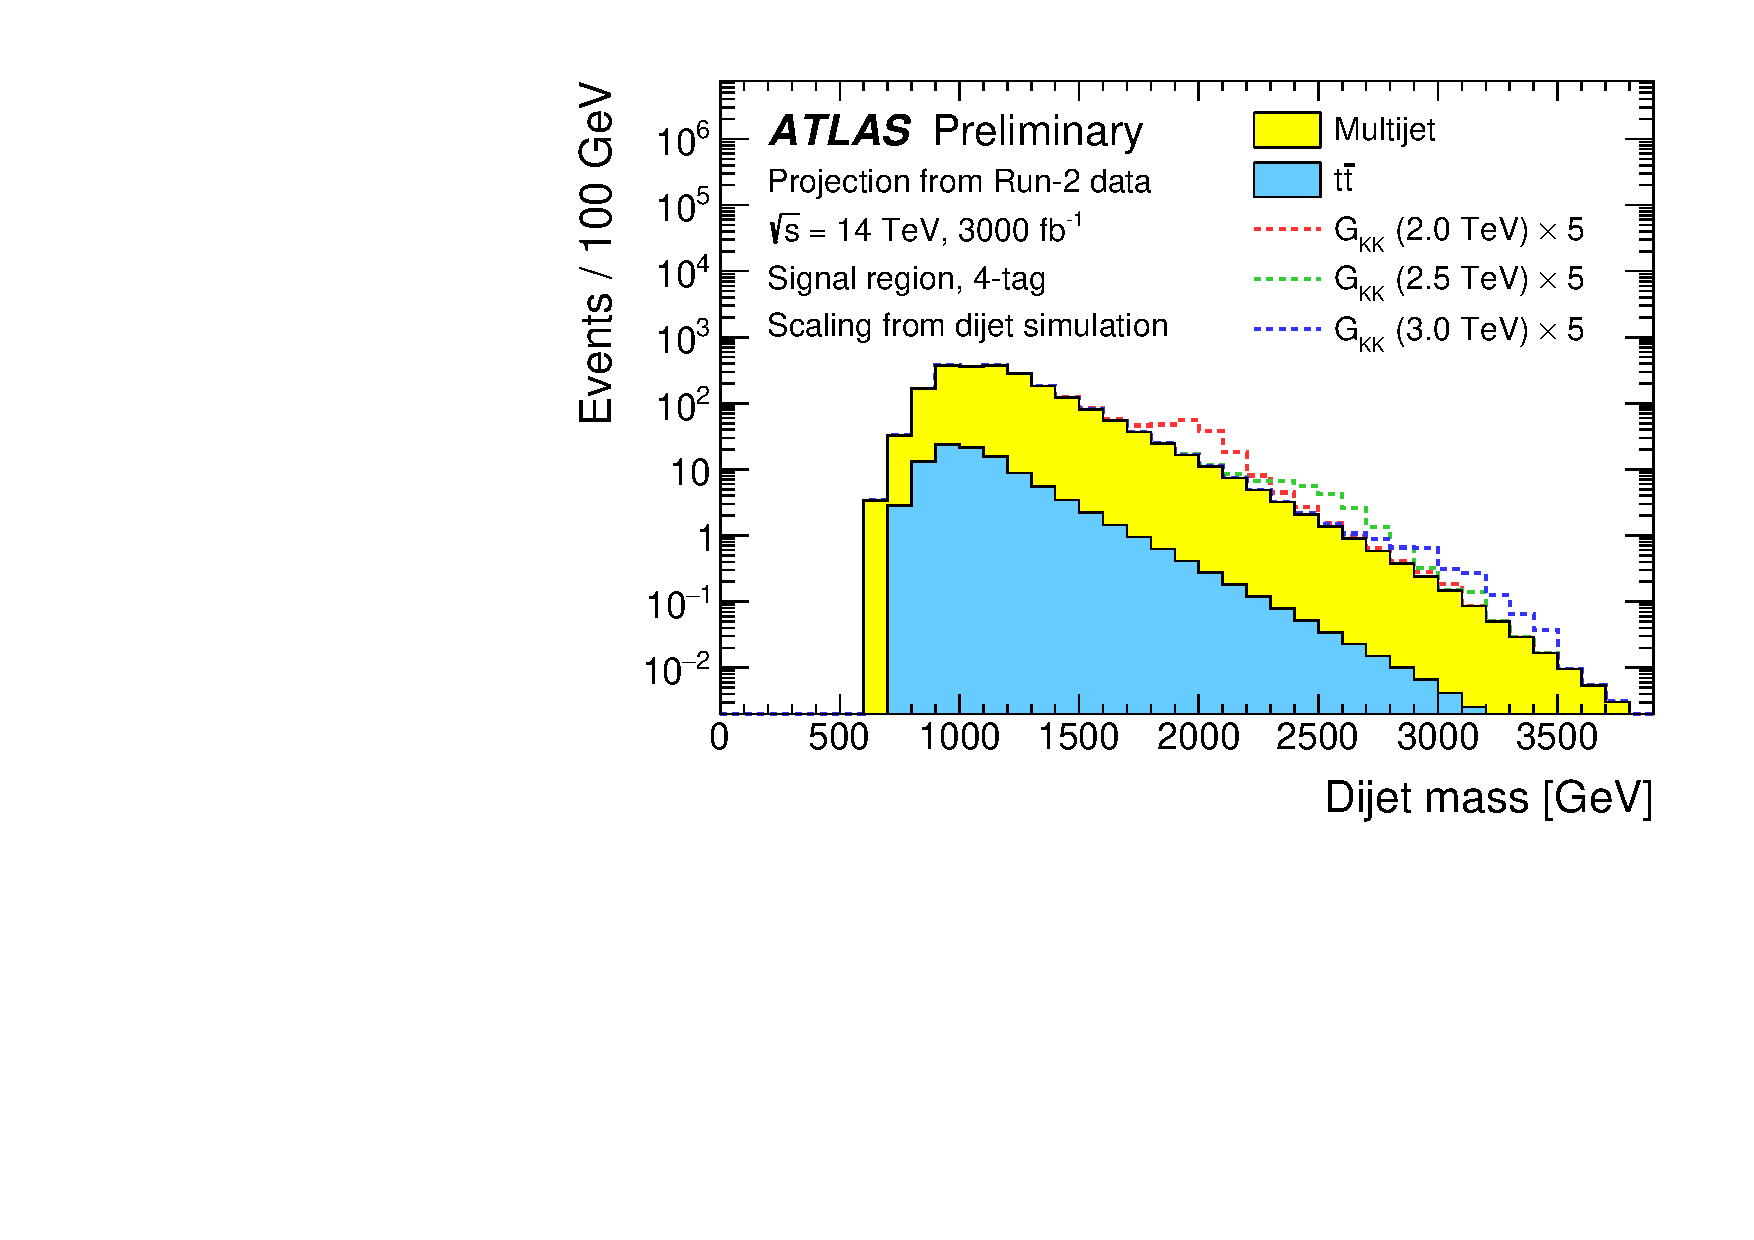
\includegraphics[width=0.48\textwidth]{\main/section7OtherSignatures/img/m_JJ_4tag_SR_rs14_13tevAnaSignals_dijetScaling_overlay}
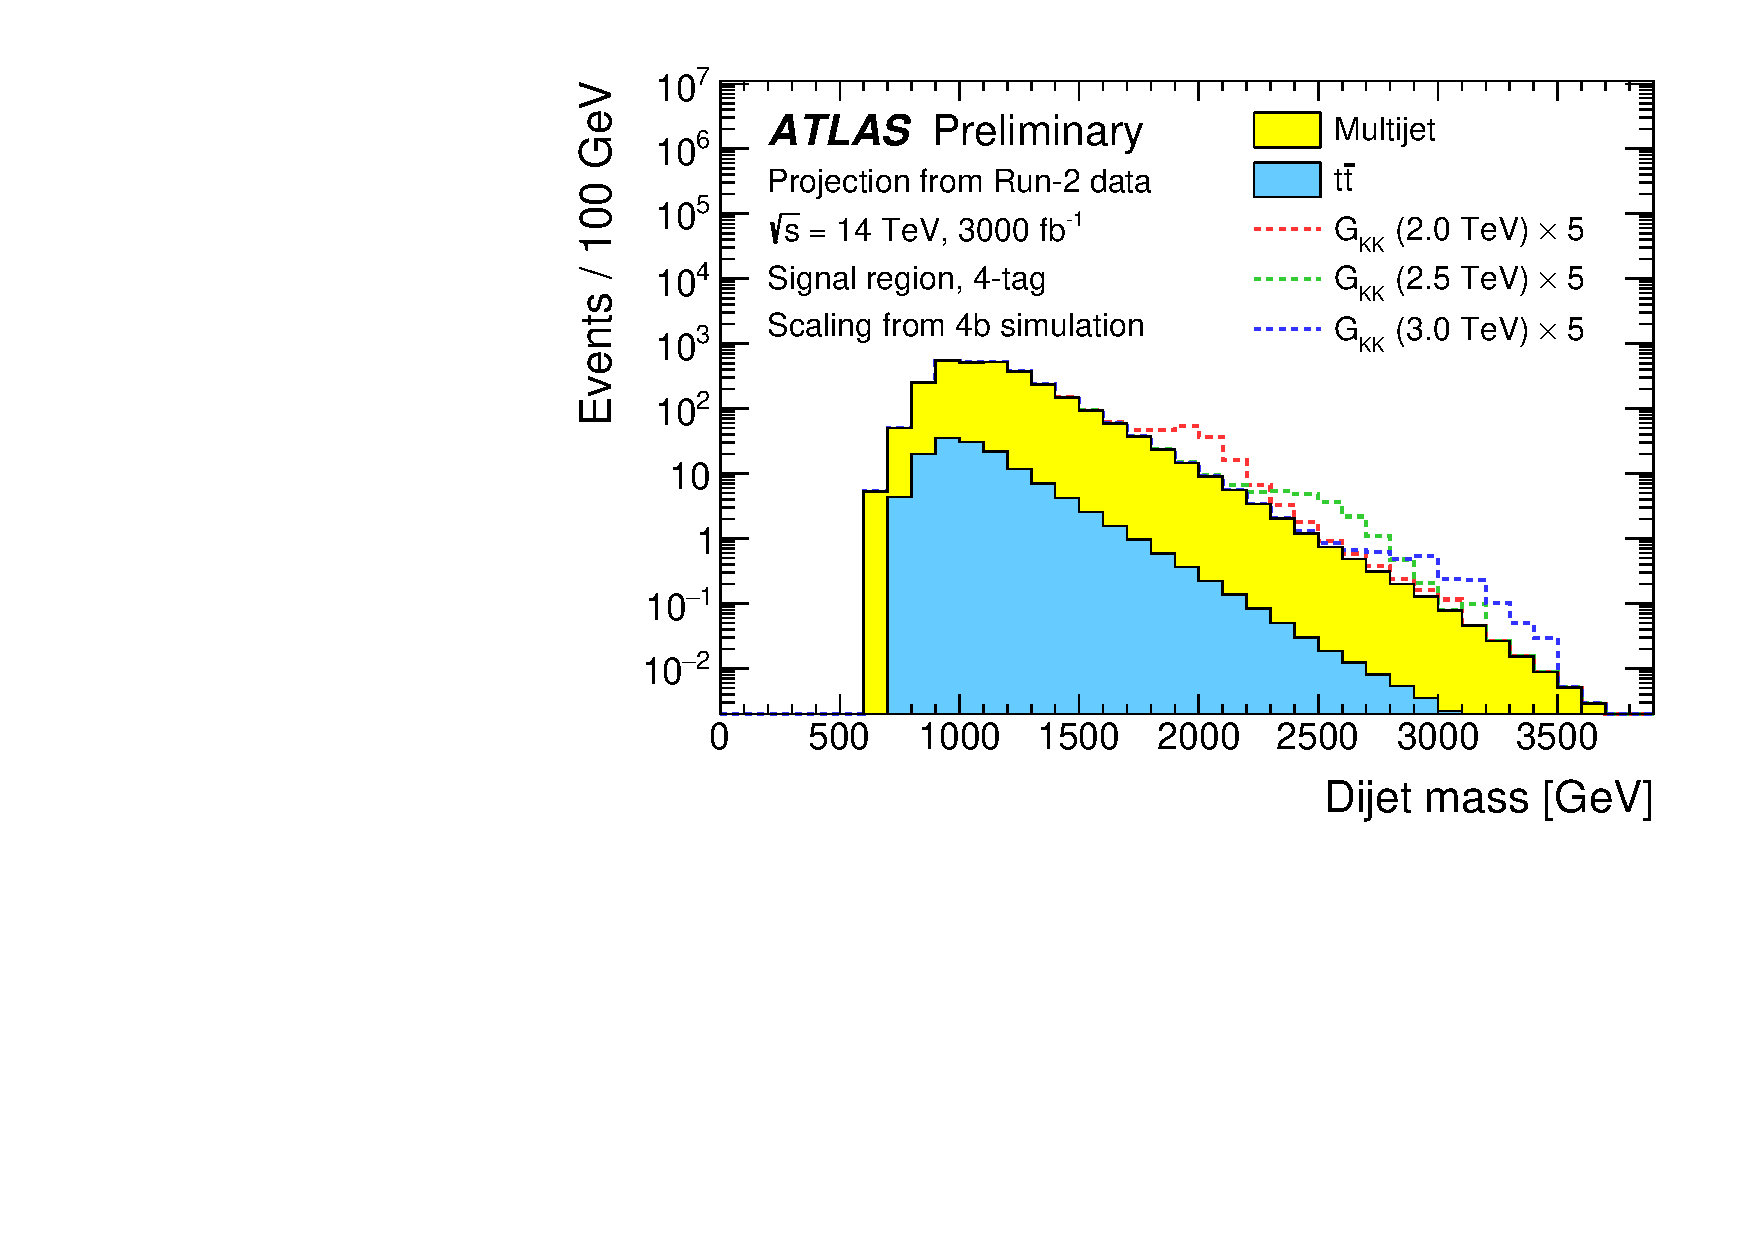
\includegraphics[width=0.48\textwidth]{\main/section7OtherSignatures/img/m_JJ_4tag_SR_rs14_13tevAnaSignals_4bScaling_overlay}
\caption{Dijet mass distributions from the truth-level analysis for 4-tag events in the signal region
 for the expected background and signals at the HL-LHC. The multijet background is scaled using
 either the dijet (left) or the $4b$ multijet (right) MC samples. The event yields for signal events
 at $G_\mathrm{KK}$ masses of 2.0, 2.5, and 3.0~TeV are scaled up for visibility.}
\label{fig:mJJ_SR_14TeV_HHatlas}
\end{center}
\end{figure}
%The full set of systematic uncertainties from the 13~TeV data analysis is
%included in the statistical analysis for the signal models. These comprise theoretical uncertainties
%in the signal acceptance as well as experimental uncertainties, which are dominant, affecting the large-$R$
%jet reconstruction (both scale and resolution uncertainties in the jet energy and mass) 
%and the $b$-tag efficiencies. Also included are uncertainties in the shape and normalization
%of the multijet and $\ttbar$ backgrounds.
%For the background, the HL-LHC extrapolation assumes that
%the background estimate uncertainties are fully driven by the statistical uncertainties 
%in the samples used in the estimate and thus scale according to $1 / \sqrt{N}$.

%The expected 95\%~\cl cross section upper limits for the HL-LHC projection at $\sqrt{s} = 14$~TeV
%with 3000~fb$^{-1}$ are shown in \fig{fig:xslimits} either the dijet (left) or the $4b$ multijet (right) 
%MC samples. 

Upper limits on $\sigma \times \cal{B}$ at $\sqrt{s} = 14$~TeV range from 1.44~fb (1.82~fb)
at a mass of 1.0~TeV to 0.025~fb (0.040~fb) at a mass of 3.0~TeV when dijet ($4b$) scaling and
the variable-radius track jets with a maximum requirement on the number of charged particles are applied.
The benefit from the use of variable-radius track jets becomes significant at the highest resonance
masses considered here, with an improvement in the upper limits of at least 24\% (depending on the
choice of scaling) at 3.0~TeV.
The additional requirement on the maximum number of charged particles further improves the upper limits 
by factors of about 20\% and 45\% at masses of 2.0 and 3.0~TeV, respectively.
Systematic uncertainties have a modest impact on the limits with an effect of at most 20\% at
1.0~TeV\ and decreasing to $\sim 5$\% at high mass.
%A hypothetical relative improvement of 10\% in the $b$-tagging efficiency for true $b$-jets with 
%unchanged charm- and light-jet rejection yields improvements in the limits
%of at most 12\% when $4b$ scaling is assumed, with more modest gains when dijet scaling is assumed.
The lower mass limits on KK gravitons are summarized in \tabb{tab:MassLimits_HH4b_ATLAS}, evaluated at the 95\%~\cl, 
 using either the dijet MC samples or the $4b$ multijet MC samples to model the changes in the 
multijet background relative to the background predictions from the 13~TeV data analysis. 

\begin{table}[htb]
\begin{center}
\begin{tabular}{lccc}
\hline
Model\T & $\sqrt{s} = 13$~TeV, 36.1~fb$^{-1}$  & \multicolumn{2}{c}{$\sqrt{s} = 14$~TeV, 3000~fb$^{-1}$} \\
        & as in \citeref{Aaboud:2018knk} &  dijet scaling & $4b$ scaling \\  % & Syst. Unc. scenario 2 \\
\hline
$\kMPl = 0.5$ \T\B &  no limit   & 2.15~TeV  & 2.00~TeV \\
$\kMPl = 1.0$ \T\B &  1.36~TeV  & 2.95~TeV  & 2.75~TeV \\
\hline
\end{tabular}
\label{tab:MassLimits_HH4b_ATLAS}
\end{center}
\caption{Expected 95\%~\cl lower limits on $G_\mathrm{KK}$ mass for the 13~TeV data analysis and
 the extrapolation to the HL-LHC for $\kMPl = 0.5$ and $1.0$ in the bulk RS model.
 Different extrapolations are provided based on modeling of the changes in multijet background using
 either the dijet or the $4b$ multijet MC samples.}
\end{table}














